\documentclass[a4paper,12pt]{article}
\usepackage[utf8]{inputenc}
\usepackage[brazilian]{babel}
\usepackage[top=3cm, left=3cm, right=2cm, bottom=2cm]{geometry}
\usepackage{graphicx}
\title{Projeto DowJones Skins}
\author{Andrey Camargo Lacerda, Fabrício Ernesto dos Santos, Guilherme Oliveira de Souza Leão, Luis Antonio Gonçalves Novaes Angelim, Vitor Urdiali}

\begin{document}
    \setlength{\parindent}{1.25cm}

    \section{1$^{\circ}$ Sprint}
    O primeiro sprint consistiu na preparação do repositório do projeto, com a instalação dos seguintes
    FrameWorks: Code Climate, Cucumber, Jest, Travis CI. Além da configuração dessas ferramentas,
    foi desenvolvido o primeiro esboço do projeto do projeto para inserção no Heroku e teste da configuração.
    Neste esboço, foi criado a Home do site e o arquivo node.js principal. Para a parte de ES4A4,
    foi criado o projeto no PivotalTracker, a fim de inserirmos as User Stories.

    \subsection{Criação do Repositório no Git}
    O primeiro passo tomado pela equipe foi a criação do repositório no Git. Para isso, o integrantes
    Guilherme Leão criou o repositório no GitHub, e posteriormente adicionou todos os membros
    da equipe e o professor de ES4A4, Daniel Morais.\\
    \begin{figure}[!htb]
        \centering
        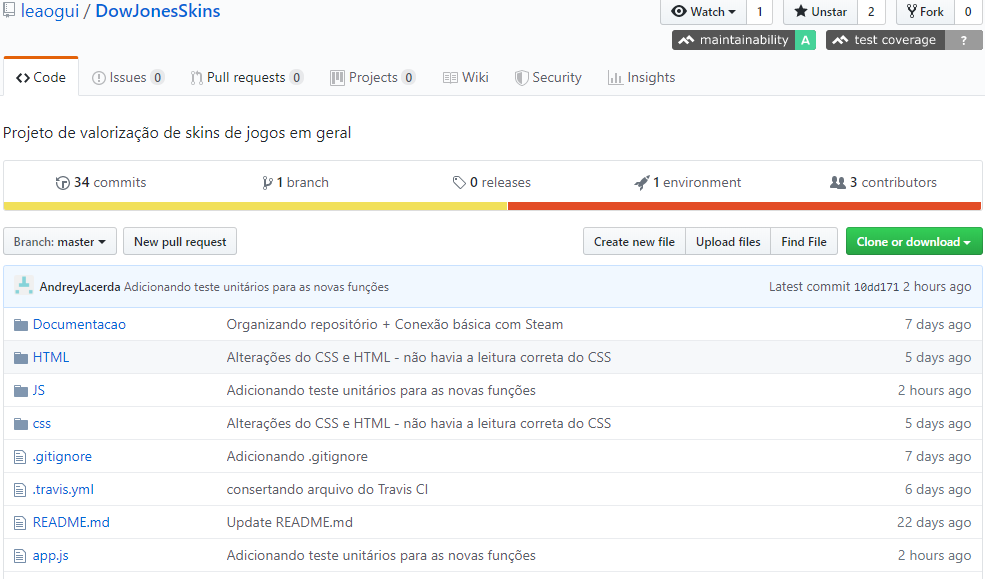
\includegraphics[scale=0.6]{Imagens/Repositorio.png}
        \caption{Repositório do Projeto no GitHub}
    \end{figure}

    \subsection{Instalação dos Frameworks}
    Dentro da pasta raíz do projeto, executamos o comando 'npm init' via CMD. Para isso, instalamos o Node.js
    em nossas máquinas. Este comando criou três arquivos: node\_modules, que consiste no diretório onde todos
    os módulos e bibliotecas utilizadas são salvas; package.json, que consiste em um 'arquivo de configuração',
    possuindo informações sobre a execução do project; package-lock.json, que consiste em um arquivo que salva
    informações de todas as biliotecas e dependencias instaladas no projeto.
    
    Com esses três arquivos criados, instalamos o Jest, a partir do comando 'npm install jest', e o Cucumber, a partir
    do comando 'npm install cucumber'. Ambos os frameworks são utilizados para testes.

    Após instalarmos os dois frameworks para o node.js, instalamos os dois frameworks para o próprio repositório do GitHub.
    O primeiro foi o CodeClimate. Para isso, o dono do repositório instalou a extensão CodeClimate no navegador,
    e posteriormente entrou no git do projeto. Dentro do GitHub do projeto, uma opção apareceu para adicionar
    o projeto ao CodeClimate. Após clicar na opção, o repositório foi lido e adicionado ao CodeClimate, 
    que agora é o plugin de avaliação de código do repositório.

    Após isso, o dono do repositório instalou o Travis CI pelo próprio 'GitHub MarketPlace'. Este framework ainda será melhor explorado,
    por enquanto apenas foi instalado.

    \subsection{Criação e configuração do Heroku}
    Para criarmos o app no Heroku, instalamos o Heroku CLI em nossas máquinas. Com ele instalado, executamos o comando
    'heroku create'. Após criar o Heroku App, entramos no web do Heroku, fizemos o login e configuramos o deploy do Heroku
    para que ele seja sincronizado com o 'push' para o repositório no GitHub.\\
    \begin{figure}[!htb]
        \centering
        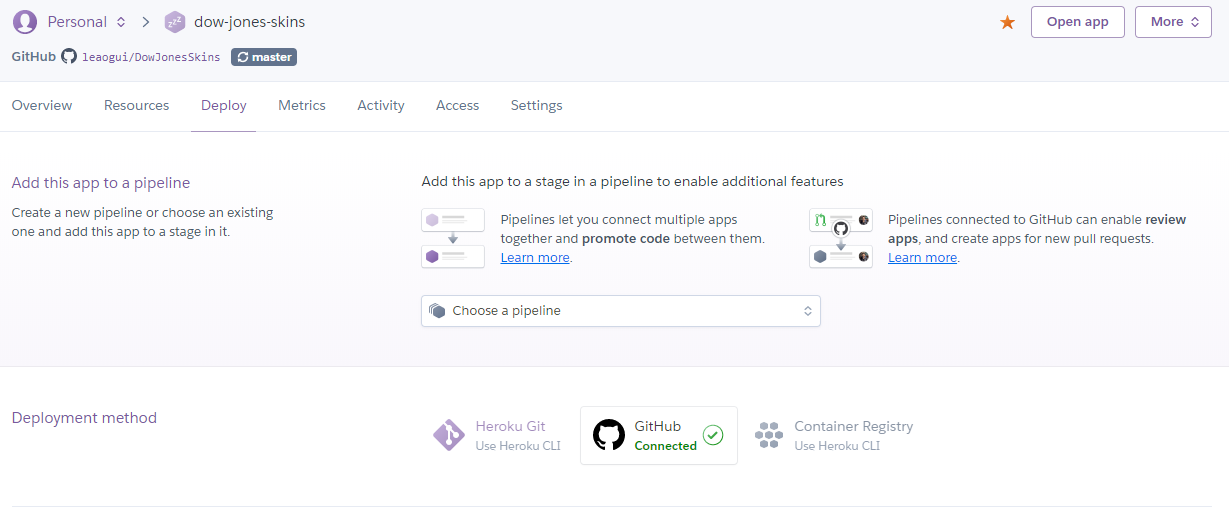
\includegraphics[scale=0.5]{Imagens/Heroku.png}
        \caption{App do Projeto no Heroku}
    \end{figure}

    \subsection{Home.html + app.js}
    Para criar o esboço da Home do projeto, utilizamos HTML, JS e CSS. Para estilização, utilizamos o Bulma,
    que consiste num FrameWork de CSS. Separamos cada arquivo em pastas baseadas em suas extensões. 
    Com isso, criamos uma pasta HTMl, uma CSS e uma JS. Na pasta CSS, jogamos o .min.css do Bulma, para que 
    pudessemos utilizá-lo.

    Com a Home criada, partimos para o primeiro contato com o login via Steam. Para isso, utilizamos a API
    da Steam para Node.JS. No arquivos app.js, que consiste no arquivo 'main', criamos todas as rotas
    e executamos o app via express. Neste arquivo, colocamos as rotas da API Steam, além de configurar
    o middleware, informação a API Key e domínio. Como executaremos tanto em local como no Heroku, modularizamos
    em vários arquivos JS com functions que realizam essa troca de domínio, porta e API Key, já que temos
    uma key apra cada domínio (local e Heroku). 

    Para esas funções foram criadas testes unitários utilizando o Jest. Esses testes estão na subpasta 'tests' 
    dentro da pasta 'JS'.

    Com tudo isso feito, finalizamos a parte de desenvolvimento.\\
    \begin{figure}[!htb]
        \centering
        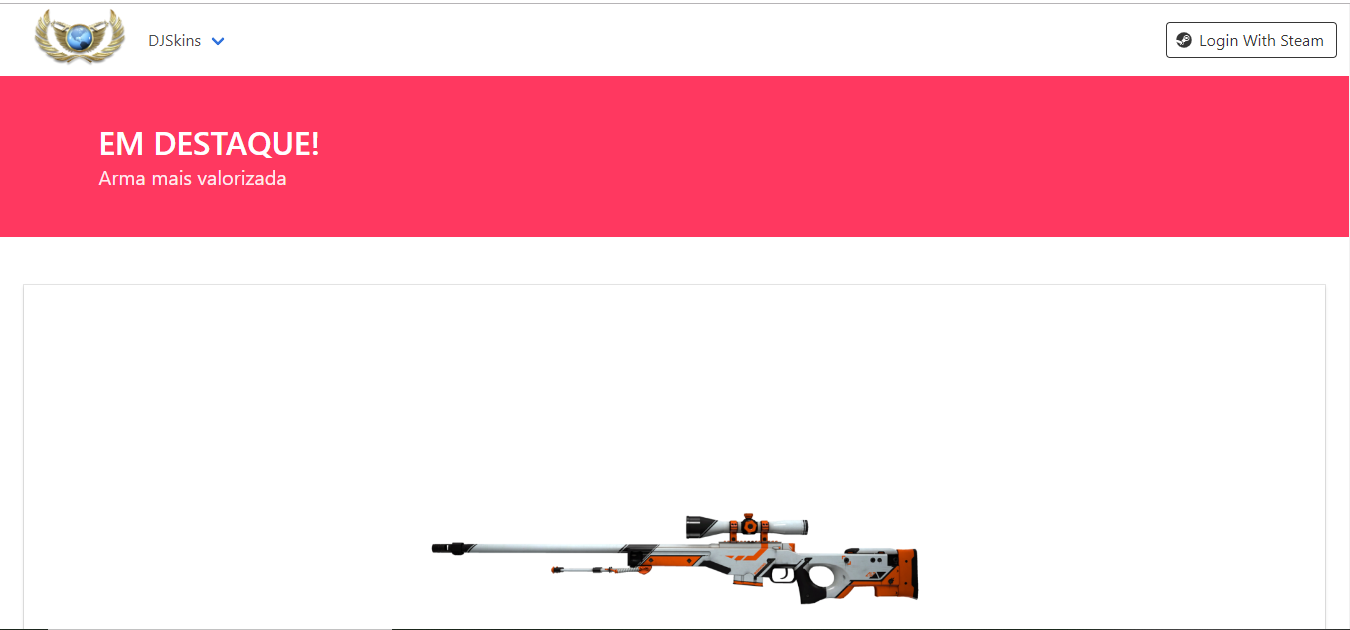
\includegraphics[scale=0.5]{Imagens/Home.png}
        \caption{Esboço da Home pronto}
    \end{figure}

    \subsection{Engenharia de Software}
    No PivotalTracker criado pelo professor Daniel, inserimos as primeiras User Stories. Essas Stories consistem 
    nas principais funcionalidades de usuários que conseguimos identificar e dividir até então. Após inserirmos, 
    Demos a pontuação para cada uma, a partir de um debate, onde o integrante que deu a menor nota defendia seu argumento 
    junto ao integrante de deu a maior nota. O melhor argumento decide a nota.

    Após isso, organizamos a prioridade e dependencias de cada User Story, além de jogarmos uma no IceBox, que 
    consistia na funcionalidade de integrar o site com o PayPal.\\
    \begin{figure}[!htb]
        \centering
        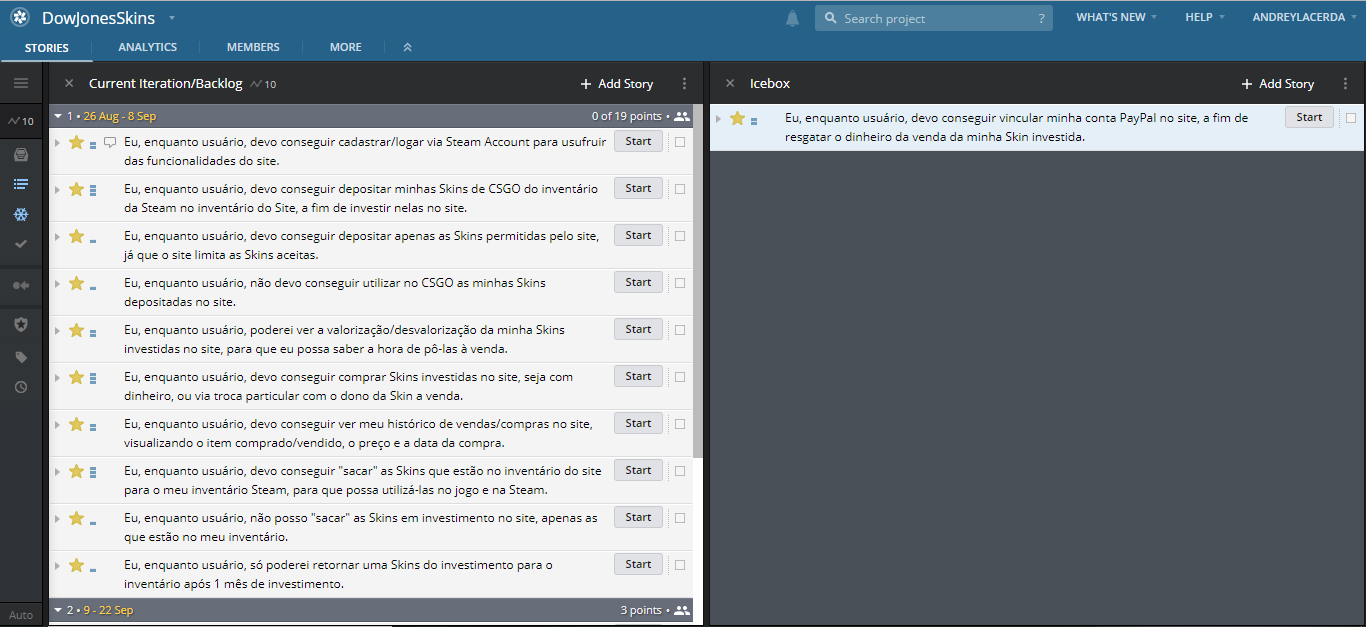
\includegraphics[scale=0.4]{Imagens/Pivotal1.png}
        \caption{PivotalTracker no 1$^{\circ}$ Sprint}
    \end{figure}

    \section{2$^{\circ}$ Sprint}
    \subsection{Descrevendo as features com Cucumber}
    Com as User Stories definidas, o passo seguinte foi esboçar todas as features utilizando o ideal do BDD 
    e utilizando o Cucumber para isso. Com isso, baseando-nos no projeto exemplo mostrado pelo professor Daniel, 
    mais a própria documentação do Cucumber, descrevemos os possíveis cenários de todas as User Stories até então.
    
    Como Dito anteriormente, para isso utilizamos a sintaxe do Cucumber, e separamos acada feature em um arquivo diferente, 
    e salvamos em uma pasta separada, chamada 'Features'. 
    Como sintaxe, declaramos cada User Storie como Feature, descrevemos ela, informamos o Background, e assim os Scenarios.

    \subsection{Testando cadastro/login com Postgre do Heroku}
    Para começar o sistema de cadastro/login, adicionamos o add-ons do PostGre ao Heroku via Heroku CLI. Para isso, 
    usamos o comando 'npm install pg' para instalar o Postgres do projeto. Após isso, adicionamos o add-on do Postgre 
    Heroku via CMD, com comando 'heroku addons:create heroku-postgresql:hobby-dev'. Após isso, seguimos os passos 
    que estão na documentação do Heroku Postgre, encontrada em 'https://devcenter.heroku.com/articles/heroku-postgresql'.

    Após isso, criamos as tabelas via CMD, usando comando 'heroku psql' e adicionando todas as linhas de comando sql.
    Tendo a conexão estável e as tabelas criadas, criamos uma classe chamada 'UserCRUD', e nela utilizamos o json 
    enviado pela Steam após conexão para salvar um Usuário no banco de dados.

    Nessa classe, a função signUp() recebe o json da Steam, conecta ao banco de dados e verifica se este usuário 
    já foi cadastro. Se sim, mais nada é feito, mas caso contrário, o usuário é inserido no banco de dados.
    Tendo isso feito, finalizamos a primeira parte do sistema de cadastro/login.

    \subsection{Estabelecendo Sessão}
    A fim de estabelecer o sistema de login, decidimos utilizar sessão para bloquear o acesso de usuário a 
    determinadas páginas do site. Para isso, utilizamos a constante Session da biblioteca 'Express', que está 
    sendo utlizada para instanciar um Servidor Web.

    Utilizamos o comando app.use() para usar o Session. Neste etapa, inserimos um id para a sessão dentro do 
    parâmetro de inicialização 'secret', e colocamos false nos outros dois itens de inicialização, saveUninitialized e resave, que, 
    após pesquisar, percebemos que não faria sentido algum.

    Após isso, colocamos dentro da página '/verify' a criação da sessão de acordo com o login do usuário na Steam. 
    Com o usuário autenticado via Steam, utilizamos o comando 'req.session.user' e atribuimos o JSON fornecido pela Steam 
    à essa constante.

    Com isso, criamos nossa sessão para cada usuário logado, e após isso, para bloquear o acesso à páginas sem que o user 
    esteja logado, inserimos um 'IF' em cada get do servidor (ignorando a /index e a /login). Dentro do IF, 
    inserimos '!req.session.user', mostrando que caso não exista ression, o usuário deverá ser redirecionado para a 
    tela de login da Steam, finalizando assim o ideal de sessão do site. 

    \subsection{Visualizando o inventário Steam do usário}
    Para obter acesso ao inventário Steam do usário logado, utilizamos da biblioteca 'steam-inventory-api'. 
    Inicializamos o serviço da API quando o servidor sobe. Após isso, quando o usuário se loga na Steam, ele é redirecionado para o '/verify' onde, 
    além de instanciarmos a sessão descrita anteriormente, passamos a visualizar os itens de seu inventário.
    
    Para isso, pegamos a steamId do usuário de dentro do JSON fornecido pela Steam e inserimos como um dos diversos parâmetros da API de 
    inventário. Utilizamos constantes para facilitar o preenchimentos dos outros parâmetros de inicialização, seguindo como base o 
    exemplo de uso da API fornecido em 'https://www.npmjs.com/package/steam-inventory-api'.

    Com isso, ao logar no Steam, o sistema consegue capturar todos os itens trocáveis do inventário do usário, 
    além de filtrar para o jogo 'CSGO'.

\end{document}